\documentclass[8pt, compress]{beamer}

%%% default
%\geometry{paperwidth=128mm,paperheight=96mm}

%\geometry{paperwidth=145mm,paperheight=108.75mm}
\geometry{paperwidth=175mm,paperheight=108.75mm}

%\geometry{paperwidth=150mm,paperheight=112.5mm}
%\geometry{paperwidth=160mm,paperheight=120mm}

\mode<presentation> {
  \usetheme{Warsaw}
 % \usetheme{Boadilla}  
  \setbeamercovered{transparent}
}

% make the navigation bar to disappear
\setbeamertemplate{headline}{}

%\usepackage{ucs}
%\usepackage[czech]{babel}
%\usepackage{czech}
%\usepackage[T1]{fontenc}
%\usepackage[latin2]{inputenc}
\usepackage{array}
\usepackage{times}
\usepackage{palatino}
\usepackage{graphicx}
\usepackage{mathtools}
\usepackage{verbatim}
%\usepackage{RT_woutmeshate}
\usepackage{xmpmulti}

\newcommand{\pdv}[2]{\frac{\partial{#1}}{\partial{#2}}}
\newcommand{\vect}[1]{\boldsymbol{#1}}
\newcommand{\matr}[1]{\mathbf{#1}}
\newcommand{\dI}{\text{d}}
\newcommand{\odv}[2]{\frac{\dI #1}{\dI #2}}
\newcommand{\ddv}[2]{\odv{#1}{#2}}
\newcommand{\mfpe}{\lambda_e}
\newcommand{\mfpei}{\lambda_{ei}}
\newcommand{\Zbar}{Z}
\newcommand{\nue}{\nu_{e}}
\newcommand{\nuei}{\nu_{ei}}
\newcommand{\nuscat}{\nu_{scat}}
\newcommand{\vmag}{v}
\newcommand{\vth}{v_{th}}
\newcommand{\vtwoh}{v_{2 th}}
\newcommand{\vn}{\vect{n}}
\newcommand{\E}{\vect{E}}
\newcommand{\B}{\vect{B}}
\newcommand{\omegaB}{\vect{\omega}_{B}}
\newcommand{\Ez}{E_z}
\newcommand{\qe}{q_e}
\newcommand{\me}{m_e}
\newcommand{\Te}{T_e}
\newcommand{\Ti}{T_i}
\newcommand{\ed}{n_e}
\newcommand{\kB}{k_B}
\newcommand{\fM}{f_M}
\newcommand{\fzero}{f_0}
\newcommand{\vfzero}{\vect{f_0}}
\newcommand{\fone}{{\vect{f_1}}}
\newcommand{\fonez}{f_{1_z}}
\newcommand{\vv}{\vect{v}}
\newcommand{\vvb}{\tilde{\vect{v}}}
\newcommand{\gv}{\nabla_{\vv}}
\newcommand{\gvb}{\nabla_{\vvb}}
\newcommand{\gx}{\nabla_{\vect{x}}}
\newcommand{\ft}{f}
\newcommand{\lnc}{\text{ln}\Lambda}
\newcommand{\Iohm}{\matr{J}_{Ohm}}

\newcommand{\vsp}[1]{\vspace{#1mm}}
\newcommand{\colorimportant}[1]{ {\color{purple} #1} }


%\newenvironment{variableblock}[3]{%
%  \setbeamercolor{block body}{#2}
%  \setbeamercolor{block title}{#3}
%  \begin{block}{#1}}{\end{block}}

% \begin{varblock}[4cm]{Title}
% \end{varblock}
\newenvironment<>{varblock}[2][.9\textwidth]{%
  \setlength{\textwidth}{#1}
  \begin{actionenv}#3%
    \def\insertblocktitle{#2}%
    \par%
    \usebeamertemplate{block begin}}
  {\par%
    \usebeamertemplate{block end}%
  \end{actionenv}}

\newcommand\myheading[1]{%
  \par\bigskip
  {\large\bfseries#1}\par\smallskip}

%%%%%%%%%%%%%%%%%%%%%%%%%%%%%%%%%%%%%%%%%%%%%%%%%%%%
%%%                pcolumn                       %%%
%%%%%%%%%%%%%%%%%%%%%%%%%%%%%%%%%%%%%%%%%%%%%%%%%%%%

\newenvironment{pcolumn}[1]{
  \begin{minipage}{#1\textwidth}
  \begin{center}
}{
  \end{center}
  \end{minipage}
}
  
%%%%%%%%%%%%%%%%%%%%%%%%%%%%%%%%%%%%%%%%%%%%%%%%%%%%
%%%                mycaptionfig                     %%%
%%%%%%%%%%%%%%%%%%%%%%%%%%%%%%%%%%%%%%%%%%%%%%%%%%%%
% \mycaptionfig - replacement for \caption
% necessary, since in multicol-environment \figure and
% therefore \caption won't work

%\newcounter{figure}
\setcounter{figure}{1}
\newcommand{\mycaptionfig}[1]{
  %\vspace{0.5cm}
  \vspace{0.05cm}
  \begin{quote}
    {{\sc Fig} \arabic{figure}: #1}
  \end{quote}
  %\vspace{1.0cm}
  \vspace{0.2cm}
  \stepcounter{figure}
}
  
\setcounter{table}{1}
\newcommand{\mycaptiontable}[1]{
  %\vspace{0.5cm}
  \vspace{0.05cm}
  \begin{quote}
    {{\sc Table} \arabic{table}: #1}
  \end{quote}
  %\vspace{1.0cm}
  \vspace{0.2cm}
  \stepcounter{table}
}
  
\useinnertheme{rectangles}
%\useoutertheme{infolines} 

\title[Multi-dimensional High-Order FEM Methods for Electron Kinetics in ALE Hydrodynamics]{Multi-dimensional High-Order FEM Methods for Electron Kinetics in ALE Hydrodynamics
%\\
%\textit{Serious Numerics for Serious Physics}
}
\author[Release number: XXXXXXXXXXXXX $\qquad\qquad$ Milan~Holec]{{\large Milan~Holec$^1$, Ben S. Southworth$^2$}}
\institute[US JAK]{
         {\large $^1$ Lawrence Livermore National Laboratory, U.S.,
		 {\it holec1@llnl.gov}
		 }\\
         {\large $^2$ University of Colorado Boulder, U.S., 
		 {\it ben.southworth@colorado.edu}
		 }
}

\date{
	\begin{figure}
    \begin{center}
	\begin{tabular}{cc} 
	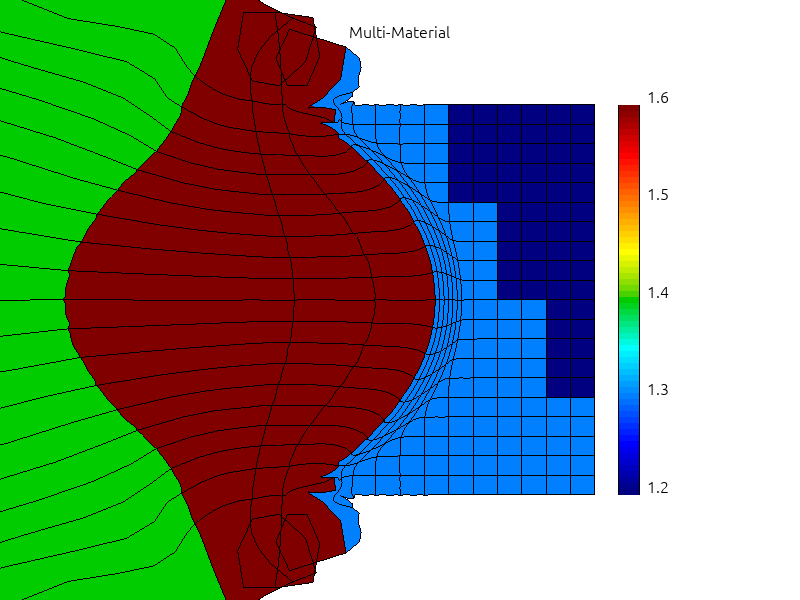
\includegraphics[width=0.3\textwidth]{../figures/material_77.png}
	&
	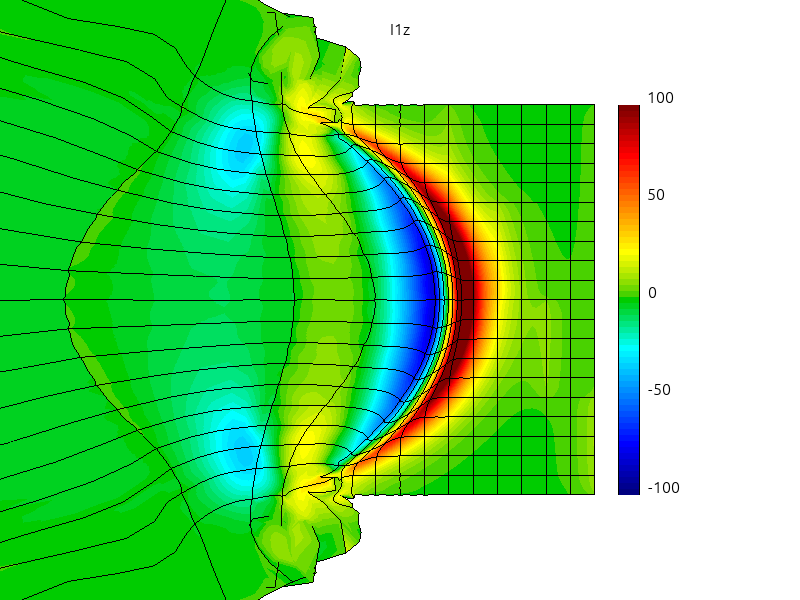
\includegraphics[width=0.3\textwidth]{../figures/nonlocalI1z_77.png}
	%&
	%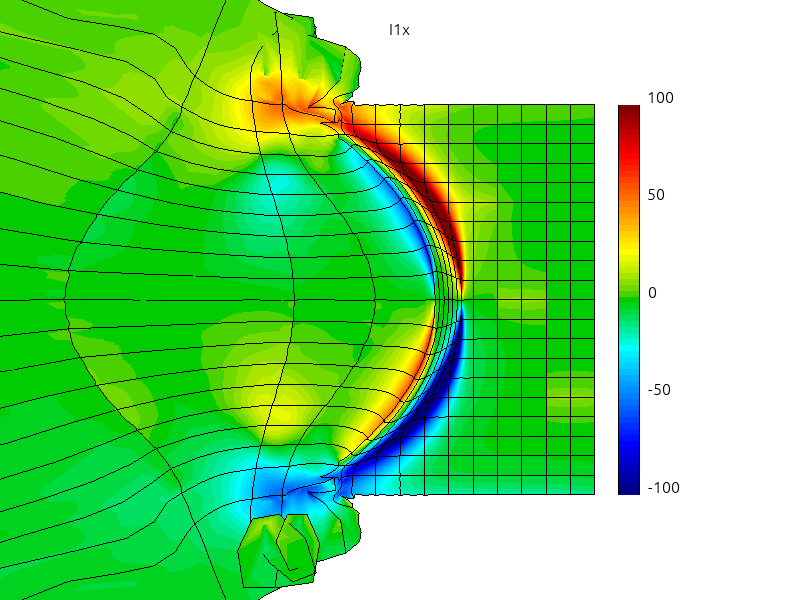
\includegraphics[width=0.3\textwidth]{../figures/nonlocalI1x_77.png}
	\end{tabular}
	\end{center}
	\end{figure}
	\begin{tabular}{c}	
	SIAM Conference on Computational Science and Engineering (CSE19)\\
	February 25 - March 1, 2019\\
	Spokane, Washington, USA 
	\end{tabular}
}
%\date{COST Working Group Meeting\\
%Advanced X-ray spatial and temporal metrology\\
%July 9-10, 2015, Madrid}      

\defbeamertemplate*{footline}{miniframes theme}%{shadow theme}
{%
  \leavevmode%
  \hbox{\begin{beamercolorbox}[wd=.5\paperwidth,ht=2.5ex,dp=1.125ex,leftskip=.3cm plus1fil,rightskip=.3cm]{author in head/foot}%
    \usebeamerfont{author in head/foot}\insertframenumber\,/\,\inserttotalframenumber\hfill
	
\includegraphics[width=0.013\textwidth]{../figures/llnl.png}\,\,\,
	\insertshortauthor
  \end{beamercolorbox}%
  \begin{beamercolorbox}[wd=.5\paperwidth,ht=2.5ex,dp=1.125ex,leftskip=.3cm,rightskip=.3cm plus1fil]{title in head/foot}% 
    \usebeamerfont{title in head/foot}\insertshorttitle 
  \end{beamercolorbox}}%
  \vskip0pt%
}      
      
\begin{document}
\begin{frame}
 \titlepage
\end{frame}

\begin{frame}
  \tableofcontents
\end{frame}

\begin{frame}
%{ \large
This document was prepared as an account of work
sponsored by an agency of the United States government.
Neither the United States government nor Lawrence Livermore National Security, 
LLC, nor any of their employees makes any warranty, expressed or implied, 
or assumes any legal liability or responsibility for the accuracy, 
completeness, or usefulness of any information, apparatus, product, 
or process disclosed, or represents that its use would not infringe privately 
owned rights. Reference herein to any specific commercial product, process, 
or service by trade name, trademark, manufacturer, or otherwise does not 
necessarily constitute or imply its endorsement, recommendation, 
or favoring by the United States government or Lawrence Livermore National 
Security, LLC. The views and opinions of authors expressed
herein do not necessarily state or reflect those of the
United States government or Lawrence Livermore National Security, LLC, 
and shall not be used for advertising or product endorsement purposes.
%}
\end{frame}

\section{Motivation - Nonlocal Magneto-Hydrodynamic model (Nonlocal-MHD)}

\begin{frame}
\begin{center}
{\huge Classical MHD}  

\begin{eqnarray}
  \text{HYDRODYNAMICS} && 
  local \rightarrow \vect{q}_e = - \kappa_{SH} \Te^{2.5} \nabla \Te \nonumber \\
  && \nonumber \\
  \frac{\dI \rho}{\dI t} &=& - \rho\nabla\cdot\vect{u} , 
  \nonumber\\ 
  \rho\, \frac{\dI \vect{u}}{\dI t} &=& - \nabla (p_i + p_e) 
  + \frac{c}{4\pi}\nabla\times\vect{B}\times \vect{B}, 
  \nonumber\\   
  \rho \left(\frac{\partial \varepsilon_i}{\partial T_i}\frac{\dI T_i}{\dI t} 
  +\frac{\partial \varepsilon_i}{\partial \rho}\frac{\dI \rho}{\dI t}\right)
  &=& 
  - p_i\nabla\cdot\vect{u} - G(T_i - T_e) , 
  \nonumber\\
  \rho \left(\frac{\partial \varepsilon_e}{\partial T_e}\frac{\dI T_e}{\dI t}
  +\frac{\partial \varepsilon_e}{\partial \rho}\frac{\dI \rho}{\dI t}\right)
  %+ \frac{\dI \epsilon_R}{\dI t} 
  &=& 
  - p_e \nabla\cdot\vect{u} 
  + \nabla\cdot\left(\kappa_{SH} \Te^{2.5} \nabla \Te \right) 
  + \sigma \E\cdot\E
  + G(T_i - T_e) + Q_{\text{IB}}(\vect{E}_L) , 
  \nonumber \\
  && \nonumber \\
  && \nonumber \\
  \text{MAXWELL EQUATIONS} && 
  resistive\rightarrow\vect{j} = \sigma \E \nonumber \\
  && \nonumber \\
  \nabla\times\vect{E} &=& -\frac{1}{c}\frac{\dI \vect{B}}{\dI t} ,
  %\quad\qquad (\text{life of magnetic field}~\vect{B}~\text{in the fluid frame})
  \nonumber \\
  \nabla\times\vect{B} &=& \frac{4\pi}{c}
  \sigma \E ,%\quad~~~ (\vect{j} \text{ depends on }f\text{ and }\vect{E}\text{ from the nonlocal model}) 
  \nonumber \\
  && \nonumber \\
  \hline \nonumber \\
  %&& \nonumber \\
  \text{KINETICS OF ELECTRONS} && Landau-Fokker-Planck \nonumber \\
  && \nonumber \\
  \pdv{f}{t} + \vect{v}\cdot\nabla f +
  \left( \vect{E} + \vect{v}\times\vect{B}\right)\cdot\nabla_{\vect{v}} f
  &=& 
  \Gamma\int \gv\gv(\vv - \vvb) \cdot \left(
  \ft\, \gvb \ft - \ft\, \gv \ft \right)\, \dI\vvb
  + \frac{\nuei}{2} \frac{\partial^2 f}{\partial \Omega^2} .
  \nonumber
\end{eqnarray}
%\let\thefootnote\relax\footnote{Spitzer and Harm, \textit{Phys. Rev.}, (1953).}
\end{center}
\end{frame}


\begin{frame}
\begin{center}
{\huge Nonlocal-MHD}  

\begin{eqnarray}
  \text{HYDRODYNAMICS} && \text{4D} \nonumber \\
  && \nonumber \\
  \frac{\dI \rho}{\dI t} &=& - \rho\nabla\cdot\vect{u} , 
  \nonumber\\ 
  \rho\, \frac{\dI \vect{u}}{\dI t} &=& - \nabla (p_i + p_e) 
  + \vect{j}(f, \vect{E}) \times \vect{B}, 
  \nonumber\\   
  \rho \left(\frac{\partial \varepsilon_i}{\partial T_i}\frac{\dI T_i}{\dI t} 
  +\frac{\partial \varepsilon_i}{\partial \rho}\frac{\dI \rho}{\dI t}\right)
  &=& 
  - p_i\nabla\cdot\vect{u} - G(T_i - T_e) , 
  \nonumber\\
  \rho \left(\frac{\partial \varepsilon_e}{\partial T_e}\frac{\dI T_e}{\dI t}
  +\frac{\partial \varepsilon_e}{\partial \rho}\frac{\dI \rho}{\dI t}\right)
  %+ \frac{\dI \epsilon_R}{\dI t} 
  &=& 
  - p_e \nabla\cdot\vect{u} - \nabla\cdot\vect{q}_e(f) 
  + \vect{j}(f, \E)\cdot\E
  + G(T_i - T_e) + Q_{\text{IB}}(\vect{E}_L) , 
  \nonumber \\
  && \nonumber \\
  && \nonumber \\
  \text{MAXWELL EQUATIONS} && \text{4D} \nonumber \\
  && \nonumber \\
  \nabla\times\vect{E} &=& -\frac{1}{c}\frac{\dI \vect{B}}{\dI t} ,
  %\quad\qquad (\text{life of magnetic field}~\vect{B}~\text{in the fluid frame})
  \nonumber \\
  \nabla\times\vect{B} &=& \frac{4\pi}{c}
  \vect{j}(f, \vect{E}) ,%\quad~~~ (\vect{j} \text{ depends on }f\text{ and }\vect{E}\text{ from the nonlocal model}) 
  \nonumber \\
  && \nonumber \\
  %&& \nonumber \\
  \text{KINETICS OF ELECTRONS} && \text{6D} \nonumber \\
  && \nonumber \\
  \vect{v}\cdot\nabla f +
  \left( \vect{E} + \vect{v}\times\vect{B}\right)\cdot\nabla_{\vect{v}} f
  &=& 
  v \tilde{\nue} \frac{\partial }{\partial v}\left(f - f_{MB}(T_e)\right)
  + \nuscat \left(\fzero - f \right) .
  \nonumber
\end{eqnarray}
\let\thefootnote\relax\footnote{M. Holec et al, \textit{Phys. Plas.}, submitted (2019) / arXiv:1901.11378 .}
\end{center}
\end{frame}

\begin{frame}
\begin{block}{AWBS electron kinetic model}
\begin{eqnarray}
  %C_V \frac{\dI T_e}{\dI t} 
  %&=& 
  %- \nabla\cdot\vect{q}_e(f) 
  %+ \vect{j}(f)\cdot\E
  %+ G(T_i - T_e) + S_H , 
  %\nonumber \\
  C_V \frac{\dI T_e}{\dI t} 
  &=& 
  - \nabla\cdot\vect{q}_e(f) 
  + \vect{j}(f)\cdot\E
  + S_H , 
  \nonumber \\
  \vect{v}\cdot\nabla f +
  \left( \vect{E} + \vect{v}\times\vect{B}\right)\cdot\nabla_{\vect{v}} f
  &=& 
  v \tilde{\nue} \frac{\partial }{\partial v}\left(f - f_{MB}(T_e)\right)
  + \nuscat \left(\fzero - f \right) .
  \nonumber
\end{eqnarray}
\end{block}
\begin{itemize}
  \item C7 (S$_N$ - discontinuous Galerkin FEM)
\begin{equation}
  \vn\cdot\nabla f + \frac{\E\cdot\vn}{\vmag} \pdv{f}{\vmag} 
  + \frac{E_\phi 
  - \vmag~B_\theta}{\vmag^2}\pdv{f}{\phi}
  + \frac{E_\theta + \vmag~B_\phi}
  {\vmag^2\sin(\phi)}\pdv{f}{\theta}
  = 
  \tilde{\nue} \frac{\partial }{\partial v}\left(f -\fM\right)
  %+ \left(\frac{\nuei}{\vmag} + \frac{\nue}{2\vmag}\right) 
  + \frac{\nuscat}{\vmag} \left(\fzero - f \right) .
  \nonumber
\end{equation}

  \item AP1 (P$_N$ (VEF $\xi=1/3$) - continuous Galerkin mixed FEM)  
      \it{Physicists like it!}
\begin{eqnarray}
  \xi\nabla\cdot\fone + \xi\frac{\qe}{\me\vmag}\E\cdot\left(
  \pdv{\fone}{\vmag} + \frac{2}{\vmag}\fone\right)
  &=& \tilde{\nue}\pdv{}{\vmag}\left(\fzero - \fM \right) , 
  \nonumber \\
  %\label{eq:AP1f0}\\
  \nabla\fzero + 
  \frac{\qe}{\me\vmag}\E\pdv{\fzero}{\vmag} 
  +\frac{\qe\B}{\me c \vmag}\vect{\times} \fone
  &=& \tilde{\nue}\pdv{\fone}{\vmag}
  - \frac{\nuscat}{\vmag}\fone 
  ,
  \nonumber \label{eq:AP1f1}
\end{eqnarray}

\end{itemize}

\end{frame}

\section{S$_N$ discontinuous Galerkin finite element approach to kinetics}
\newcommand{\fs}{0.5}

\begin{frame}
\begin{center}
{\Large S$_N$ upwind DG, parallel-Approximate-Ideal-Relaxation multi-grid solver}
%\\
%explain the concept of deceleration + necessity of using high order in vmag. 
\begin{equation}
  \matr{M}_{_{(\tilde{\nue} - \frac{\E\cdot\vn_d}{\vmag})}}\cdot 
  \frac{\Delta \vect{f}_d}{\Delta \vmag}
  =
  \left(\vn_d\cdot\matr{G} + \matr{F}_d\right) \cdot 
  \left(\tilde{\vect{f}}_d + \Delta \vect{f}_d\right) 
  ~+~ \matr{M}_{_{(\frac{\nuscat}{\vmag})}}\cdot 
  \left(\tilde{\vect{f}}_d + \Delta \vect{f}_d\right)
  ~+~ \matr{S}_{_{(\nuscat, \E, \B)}} \cdot \tilde{\vect{f}}
  ~+~ \vect{S}_{_{(\tilde{\nue}\pdv{\fM}{\vmag})}}
  %\left( - \fzero\right)
  %+ \frac{E_\phi 
  %- \vmag~B_\theta}{\vmag^2}\pdv{f}{\phi}
  %+ \frac{E_\theta + \vmag~B_\phi}{\vmag^2\sin(\phi)}\pdv{f}{\theta}
  %+ \tilde{\nue} \frac{\partial \fM}{\partial v} .
  \nonumber
\end{equation}
\begin{tabular}{c|ccccc}
    %\hline\\
    Velocity groups       & 10   & 20 & 40 & 80 & 160 \\
    \hline
	Backward Euler & 1433/204.6 & 1342/151.1 & 1290/139.7 & 1262/132.1 & 1248/127.9 \\
    SDIRK2         & 1275/133.9 & 1245/132.3 & 1237/126.1 & 1235/124.2 & 1234/123.6 \\
    SDIRK3         & 1265/90.2 & 1239/133.1 & 1235/125.1  & 1234/123.7 & 1234/123.5 \\
    %SDIRK4         &  &  &  &  & 
    %\hline
\end{tabular}
\begin{tabular}{cc}
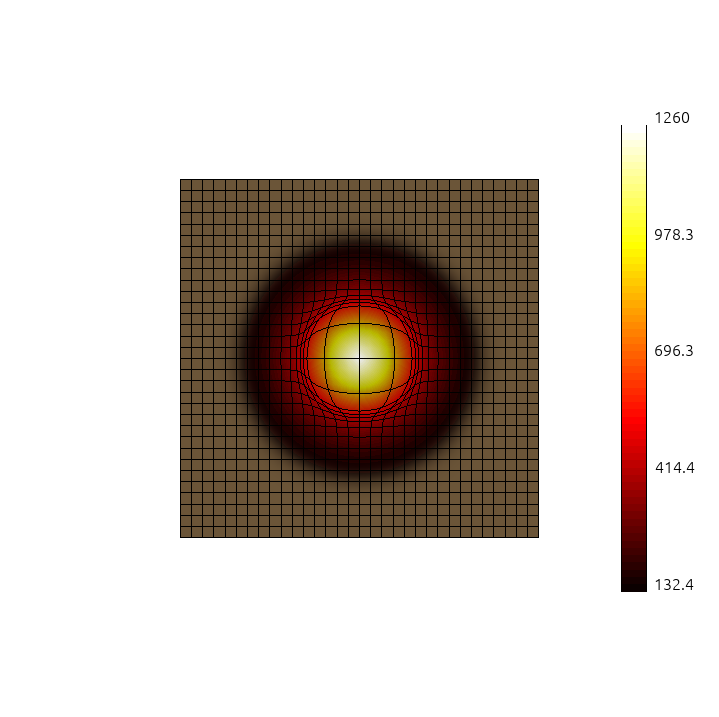
\includegraphics[width=\fs\textwidth]{../figures/ALE_Te_local_pfire.png}
&
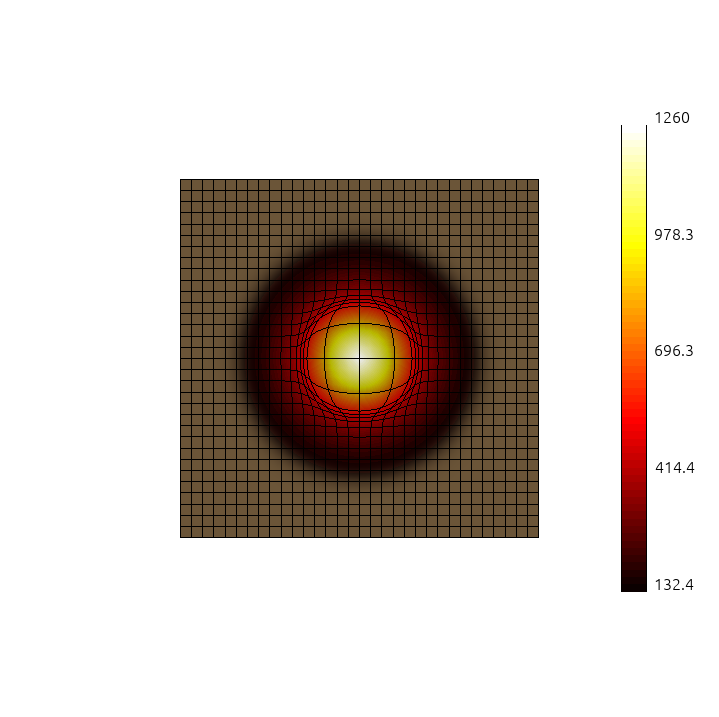
\includegraphics[width=\fs\textwidth]{../figures/ALE_Te_local_pfire.png}
\end{tabular}
\end{center}
\end{frame}

\renewcommand{\fs}{0.33}
\begin{frame}
\begin{center}
%Local + nonlocal results, pAIR stats
\begin{tabular}{cc}
Local hydro temperature & Nonlocal kinetic temperature \\
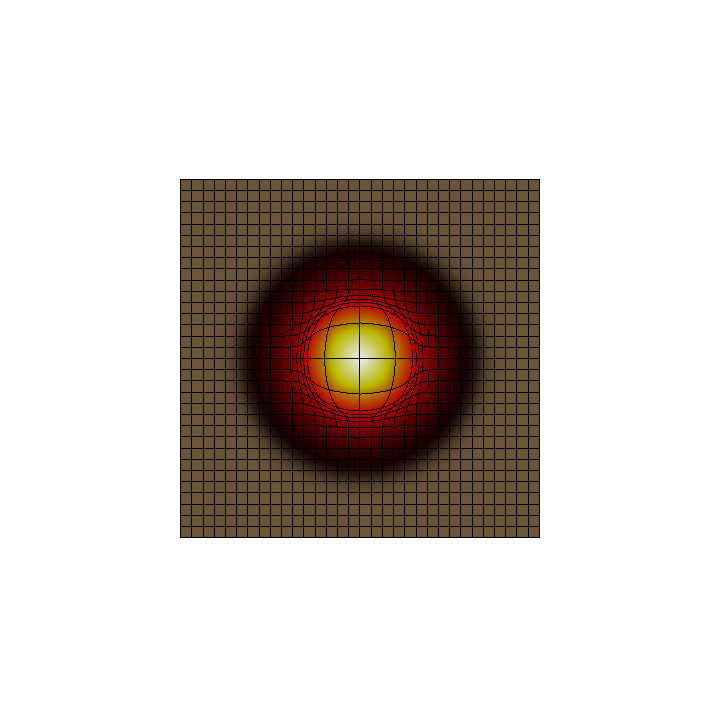
\includegraphics[width=\fs\textwidth]{../figures/ALE_Te_local_nopfire.png}
&
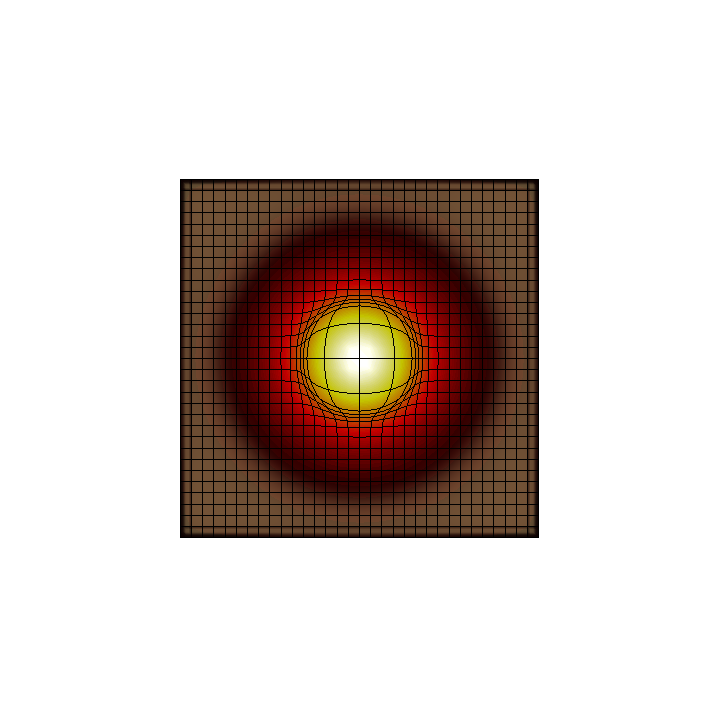
\includegraphics[width=\fs\textwidth]{../figures/ALE_Te_nonlocal32_nopfire.png}
\\
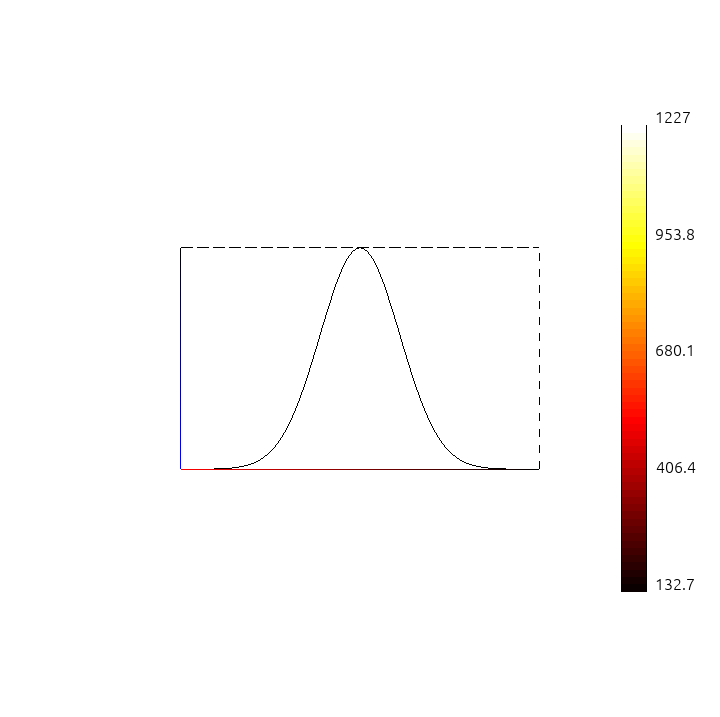
\includegraphics[width=\fs\textwidth]{../figures/ALE_Te_local1D_pfire.png}
&
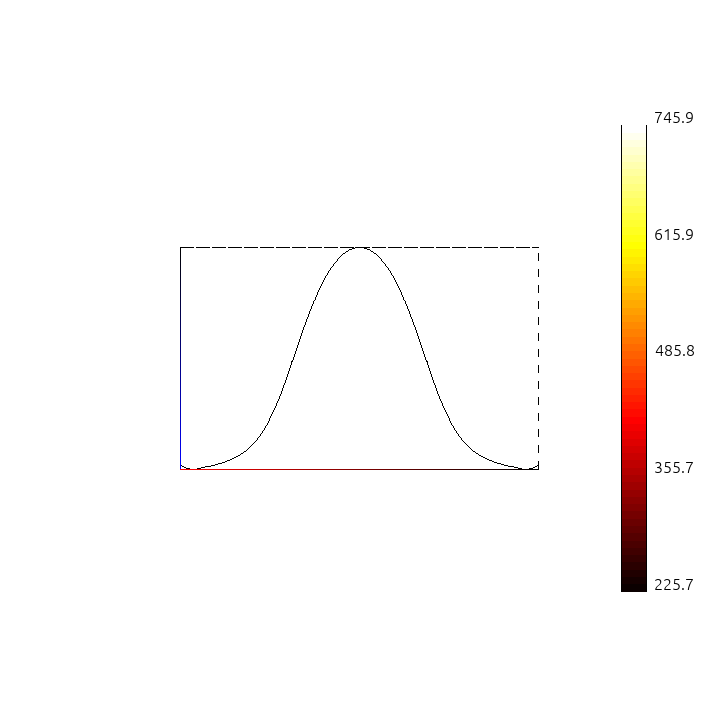
\includegraphics[width=\fs\textwidth]{../figures/ALE_Te_nonlocal1D_pfire.png}
\end{tabular}
\end{center}
\end{frame}

\section{P$_N$ mixed finite element approach to kinetics}
\newcommand{\edf}{\colorimportant{f}}
\renewcommand{\fs}{0.33}
\begin{frame}
\begin{center}
%{\huge Nonlocal electron transport regime - PIC/VFP0/AWBS}
{\Large AP1 formulation PCG(AMG), fixed P1 angular discretization}
\begin{eqnarray}
  \matr{M}^{L_2}_{_{(\tilde{\nue})}}\cdot\ddv{\vfzero}{\vmag} 
  - \matr{V}^{L_2}_{_{(\frac{\xi\qe\E}{\me\vmag})}}\cdot\ddv{\fone}{\vmag}
  &=&
  \matr{D}^{L_2}_{_{(\xi)}}\cdot\fone 
  + \matr{M}^{L_2}_{_{(\frac{\xi2\qe\E}{\me\vmag^2})}}\cdot\fone
  + \vect{S}^{L_2}_{_{(\tilde{\nue}\pdv{\fM}{\vmag})}}, 
  \nonumber\label{eq:FEMAP1f0}
  \\
  \matr{M}^{H_1}_{_{(\tilde{\nue})}}\cdot\ddv{\fone}{\vmag}
  - \matr{V}^{H_1}_{_{(\frac{\qe\E}{\me\vmag})}}\cdot\ddv{\vfzero}{\vmag}
   &=& 
  \matr{G}^{H_1}\cdot\vfzero 
  + \matr{M}^{H_1}_{_{(\frac{\nuscat}{\vmag})}}\cdot\fone 
  + \matr{C}^{H_1}_{_{(\frac{\qe\B}{\me c \vmag}\vect{\times})}}\cdot\fone
  ,
  \nonumber \label{eq:FEMAP1f1}
\end{eqnarray}

\begin{tabular}{ccc}
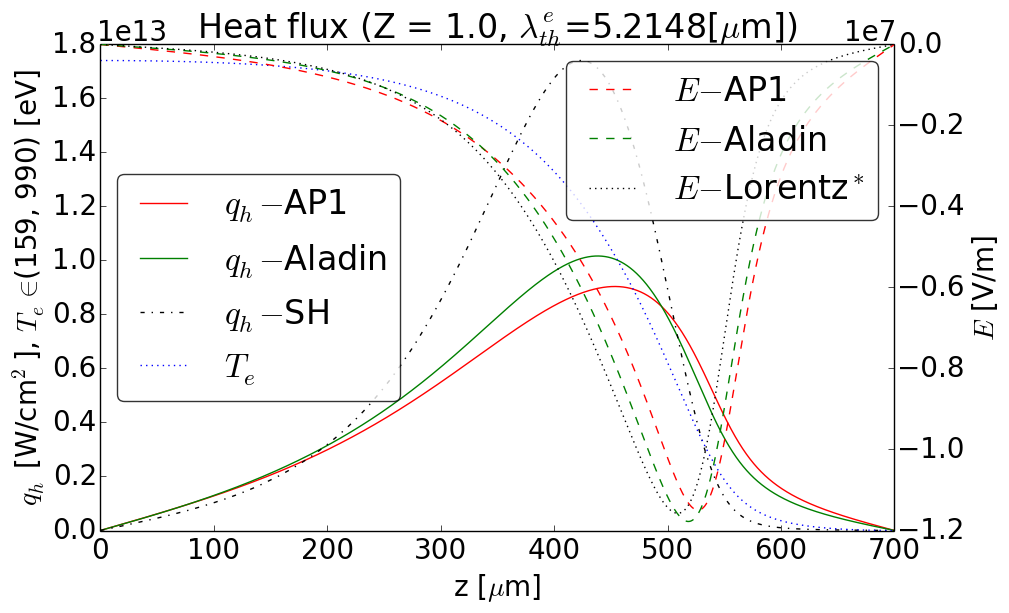
\includegraphics[width=\fs\textwidth]{../figures/C7_Aladin_case5_heatflux.png}
&
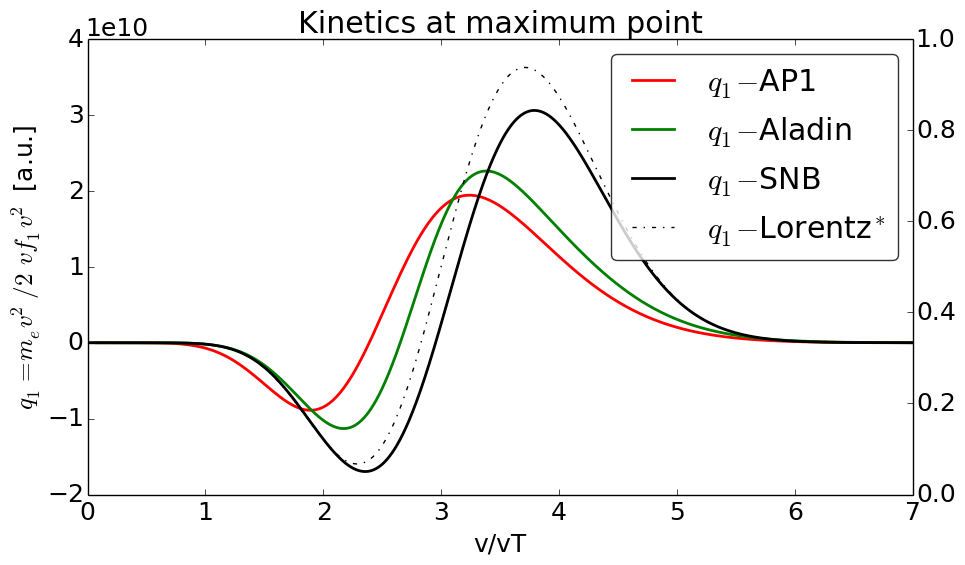
\includegraphics[width=\fs\textwidth]{../figures/C7_Aladin_case5_kinetics.png}
&
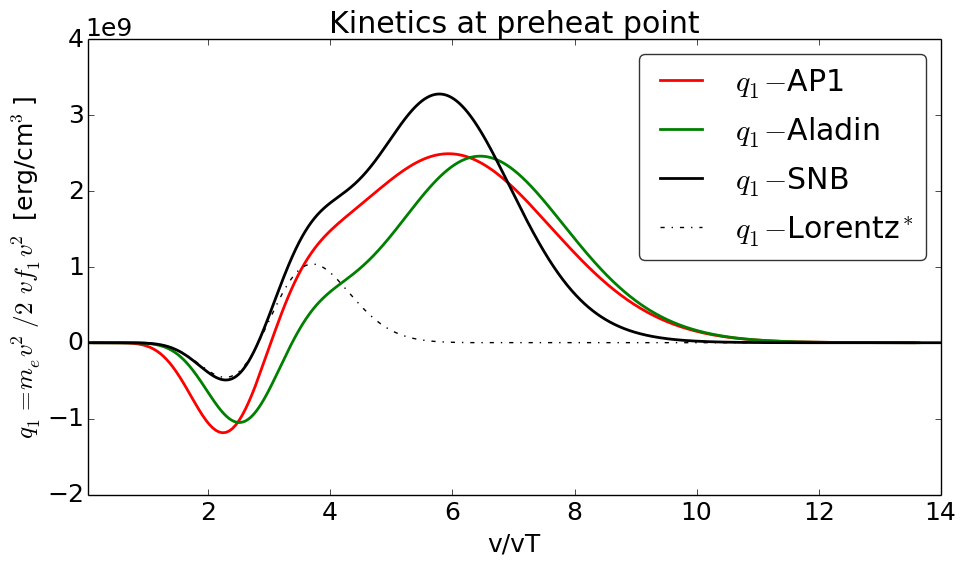
\includegraphics[width=\fs\textwidth]{../figures/C7_Aladin_case5_nonlocal_kinetics.png}
\\
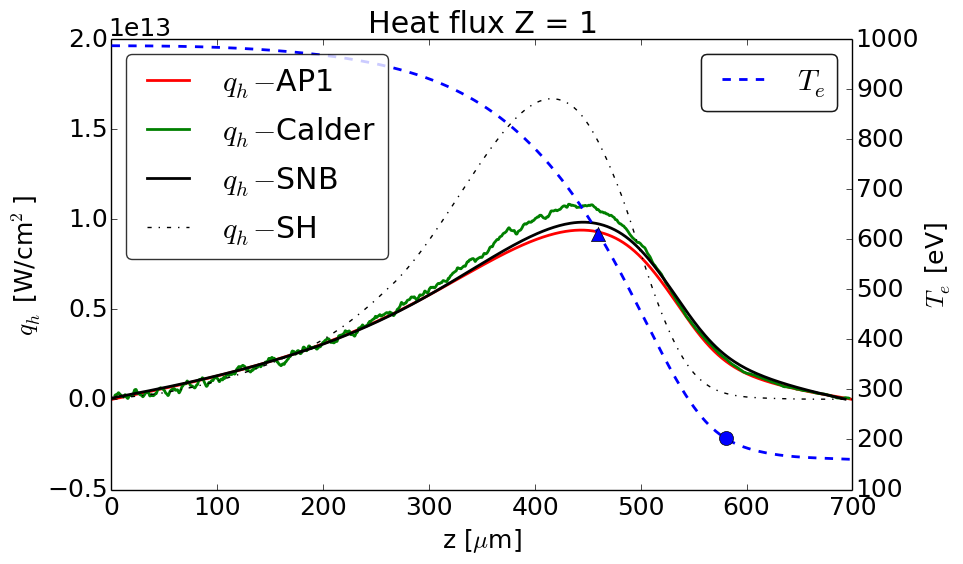
\includegraphics[width=\fs\textwidth]{../figures/C7_Calder_case5_heatflux.png}
&
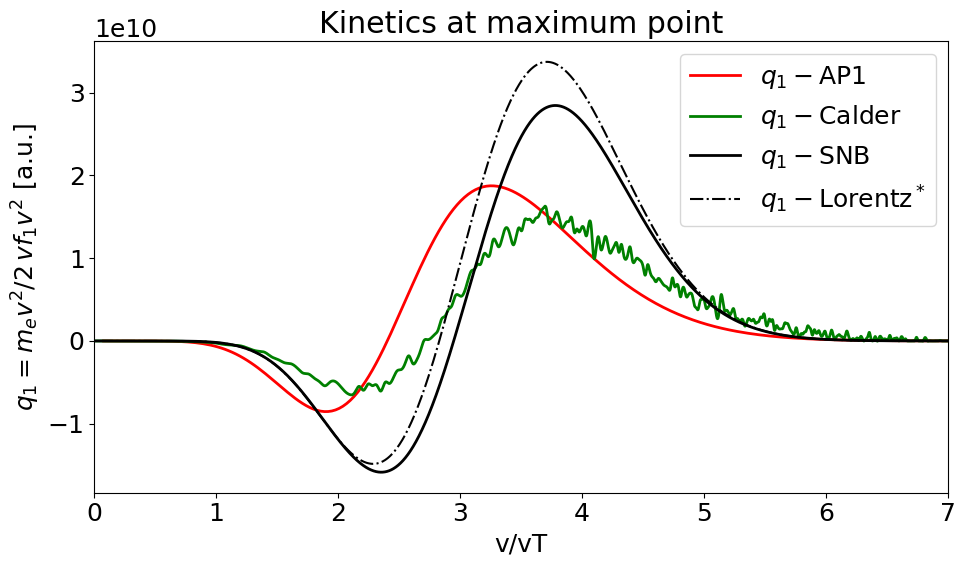
\includegraphics[width=\fs\textwidth]{../figures/C7_Calder_case5_kinetics.png}
&
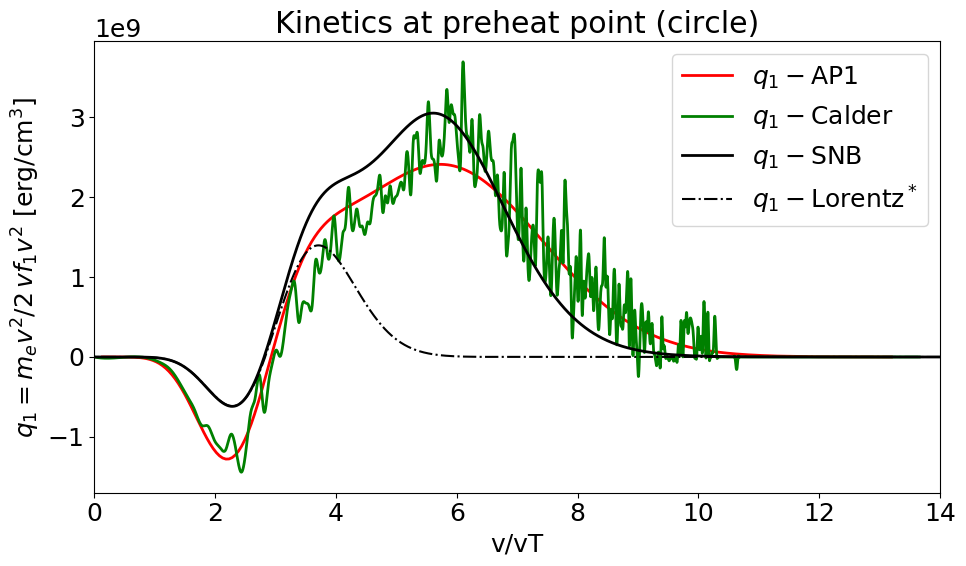
\includegraphics[width=\fs\textwidth]{../figures/C7_Calder_case5_nonlocal_kinetics.png}
\end{tabular}
\let\thefootnote\relax\footnote{M. Holec et al, \textit{Phys. Plas.}, submitted (2019) / arXiv:1901.11378 .}
\end{center}
\end{frame}

\section{Conclusions}

\begin{frame}
\begin{center}
{\Large Electron velocity limit - friction vs. $\vect{E}$ stopping}
\begin{equation}
  \left( \tilde{\nue} - \frac{\E\cdot\vn}{\vmag} \right) 
  \frac{\partial f}{\partial \vmag}
  =
  \vn\cdot\nabla f 
  + \frac{\nuscat}{\vmag} \left(f - \fzero\right)
  + \frac{E_\phi 
  - \vmag~B_\theta}{\vmag^2}\pdv{f}{\phi}
  + \frac{E_\theta + \vmag~B_\phi}{\vmag^2\sin(\phi)}\pdv{f}{\theta}
  + \tilde{\nue} \frac{\partial \fM}{\partial v} .
  \nonumber
\end{equation}

\begin{tabular}{c}
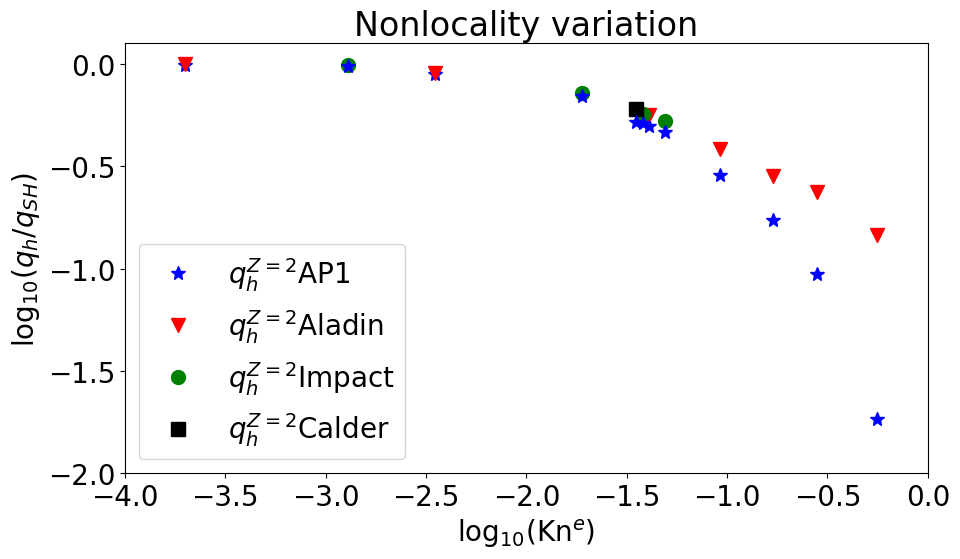
\includegraphics[width=0.5\textwidth]{../figures/Kn_results.png}
\end{tabular}

$\vect{E}$ stopping overtakes collisions for Kn$~>0.1$ .
\let\thefootnote\relax\footnote{M. Holec et al, \textit{Phys. Plas.}, submitted (2019) / arXiv:1901.11378 .}

\begin{tabular}{c|ccccc}
    \hline\hline\\
    %Kn$^e$ & $10^{-4}$ & $10^{-3}$ & $10^{-2}$ & $10^{-1}$ & $1$ \\\\
    Kn & $\,\,10^{-4}\,\,$ & $\,\,10^{-3}\,\,$ & $\,\,10^{-2}\,\,$ & $\,\,10^{-1}\,\,$ & $\,\,1\,\,$ \\\\
    \hline\\
    $v_{lim} / v_{th}$ & 70.8 & 22.4 & 7.3 & 3.1 & 1.8\\\\
    \hline\hline
\end{tabular} 
\end{center}
\end{frame}

\begin{frame}
%Scattering/temperature reaction term\\
%DSA (a full model without bending, consistent numerical scheme required 
%for the construction of the preconditioner, Ref. Terry's SIAM 2018)
%
%\begin{equation}
%  \frac{1}{\Delta \vmag}
%  \matr{M}_{_{(\tilde{\nue} - \frac{\E\cdot\vn_d}{\vmag})}}\cdot 
%  \Delta \vect{f}_d
%  =
%  \left(\vn_d\cdot\matr{G} + \matr{F}_d\right) \cdot 
%  \left(\tilde{\vect{f}}_d + \Delta \vect{f}_d\right) 
%  ~+~ \matr{M}_{_{(\frac{\nuscat}{\vmag})}}\cdot 
%  \left(\tilde{\vect{f}}_d + \Delta \vect{f}_d\right)
%  - \matr{M}_{_{(\frac{\nuscat}{\vmag})}}\cdot 
%  \left(\tilde{\vect{f}}_0 + \Delta \vect{f}_0\right)  
%  + \vect{q}   
%  \nonumber
%\end{equation}
%\begin{equation}
%  \frac{1}{\Delta \vmag}
%  \matr{M}_{_{(\tilde{\nue} - \frac{\E\cdot\vn_d}{\vmag})}}\cdot 
%  \Delta \vect{f}_d
%  =
%  \left(\vn_d\cdot\matr{G} + \matr{F}_d\right) \cdot 
%  \Delta \vect{f}_d 
%  + \matr{M}_{_{(\frac{\nuscat}{\vmag})}}\cdot 
%  \Delta \vect{f}_d
%  - \matr{M}_{_{(\frac{\nuscat}{\vmag})}}\cdot\Delta \vect{f}_0 
%  + \vect{q}   
%  \nonumber
%\end{equation}
\begin{center}
{\Large Adaptive DSA scattering preconditioner}
\begin{equation}
  \left[\left(\vn_d\cdot\matr{G} + \matr{F}_d\right) 
    + \matr{M}_{_{\left(\frac{\nuscat(\Zbar)}{\vmag}\right)}}
  - \matr{M}_{_{\left(\frac{\tilde{\nue}}{\Delta \vmag} - \frac{\E\cdot\vn_d}{\vmag \Delta \vmag}\right)}}\right]
  \cdot \Delta \vect{f}_d
  =
    \matr{M}_{_{\left(\frac{\nuscat(\Zbar)}{\vmag}\right)}}\cdot\Delta \vect{f}_0 
  + \vect{q}
  \nonumber
\end{equation}
\begin{block}{Fixed-point iteration}
\begin{equation}
  \Delta \vect{f}_0^{k+1}
  =
    \matr{A}\cdot\matr{M}_{_{\left(\frac{\nuscat(\Zbar)}{\vmag}\right)}}\cdot\Delta \vect{f}_0^k 
    + \matr{A}\cdot \vect{q}
  \nonumber
\end{equation}
\end{block}
Continuous analysis of local (Kn$\ll$1) transport regime $\rightarrow$ DIFFUSION
%\begin{equation}
%  \left(\frac{\tilde{\nue}}{\Delta \vmag} - \frac{\E\cdot\vn_d}{\vmag \Delta \vmag}\right)\Delta f_0
%  + \nabla\cdot\left(\frac{1}{3} \frac{1}{\frac{\nuscat(\Zbar)}{\vmag} - \frac{\tilde{\nue}}{\Delta \vmag} + \frac{\E\cdot\vn_d}{\vmag \Delta \vmag}}\nabla f_0 \right)
%    = q + O(\text{Kn}^2)
%  \nonumber
%\end{equation}
\begin{equation}
  \left(\frac{\tilde{\nue}}{\Delta \vmag} - \frac{\E\cdot\vn_d}{\vmag \Delta \vmag}\right)\Delta f_0
  + \nabla\cdot\left(\frac{\vmag}{3\nuscat(\Zbar)}\nabla f_0 \right)
    = q + O(\text{Kn}^2)
  \nonumber
\end{equation}
\let\thefootnote\relax\footnote{T. Haut et al, \textit{SIAM}, submitted (2018) / arXiv:1810.11082 .}
\begin{block}{A diffusion consistent $\zeta(\text{Kn})$ adaptive preconditioning 
$\matr{E} = \left[ \matr{M}
  + \zeta~ \matr{D}\right]$ with $\zeta\rightarrow 0$ for Kn$~>1$}
\begin{equation}
  \left[ \matr{M}_{_{\left(\frac{\tilde{\nue}}{\Delta \vmag} - \frac{\E\cdot\vn_d}{\vmag \Delta \vmag}\right)}}
  + \zeta~ \matr{D}_{_{\left(\frac{\vmag}{3\nuscat(\Zbar)}\right)}}\right]\cdot\Delta \vect{f}_0^{k+1}
  =
    \matr{E}\cdot\matr{A}\cdot\matr{M}_{_{\left(\frac{\nuscat(\Zbar)}{\vmag}\right)}}\cdot\Delta \vect{f}_0^k 
    + \matr{E}\cdot\matr{A}\cdot \vect{q}
  \nonumber
\end{equation}
\end{block}
\end{center}
\end{frame}

\begin{frame}
\begin{center}
{\huge Conclusions}
%\begin{block}{Collision operators}
%    \begin{eqnarray}
%        C_{FP} &=& \Gamma_{ee}\int \gv\gv(\vv - \vvb) \cdot \left(
%        \ft\, \gvb \ft - \ft\, \gv \ft \right)\, \dI\vvb
%        + \frac{\nuei}{2} 
%        \pdv{}{\mu}\left((1 - \mu^2)\pdv{f}{\mu}\right) ,
%        \\
%        C_{BGK} &=& \nue(\fM - \ft)
%        + \frac{\Zbar + 4.2}{\Zbar + 0.24}\frac{\nuei}{2} 
%        \pdv{}{\mu}\left((1 - \mu^2)\pdv{f}{\mu}\right) ,
%        \\
%        C_{FP0} &=& 
%        v \nue\frac{\partial}{\partial v}
%        \left[C(\fzero)\fzero
%        + D(\fzero)\frac{\partial \fzero}{\partial v}\right]
%        + \frac{\Zbar + 4.2}{\Zbar + 0.24}\frac{\nuei}{2} 
%        \pdv{}{\mu}\left((1 - \mu^2)\pdv{f}{\mu}\right) ,
%        \\
%        C_{AWBS} &=& \vmag \frac{\nue}{2}
%        \pdv{}{\vmag}\left(\ft - \fM\right)
%        + \frac{\nuei + \frac{\nue}{2}}{2} 
%        \pdv{}{\mu}\left((1 - \mu^2)\pdv{f}{\mu}\right).      
%    \end{eqnarray}
%\end{block}
\begin{itemize}
  \item 7D microscopic world of electrons in hydro simulations.
  \item S$_N$ high-order DG finite element approach.
  \item P$_1$ high-order mixed finite element approach.
  \item $\E$ field dominated stopping (P$_1$ fails).
  \item Adaptive scattering preconditioner (deep machine learning).
  \item pAIR scaling $\log(P)^{1.22}$.
\end{itemize}
\begin{tabular}{cc}
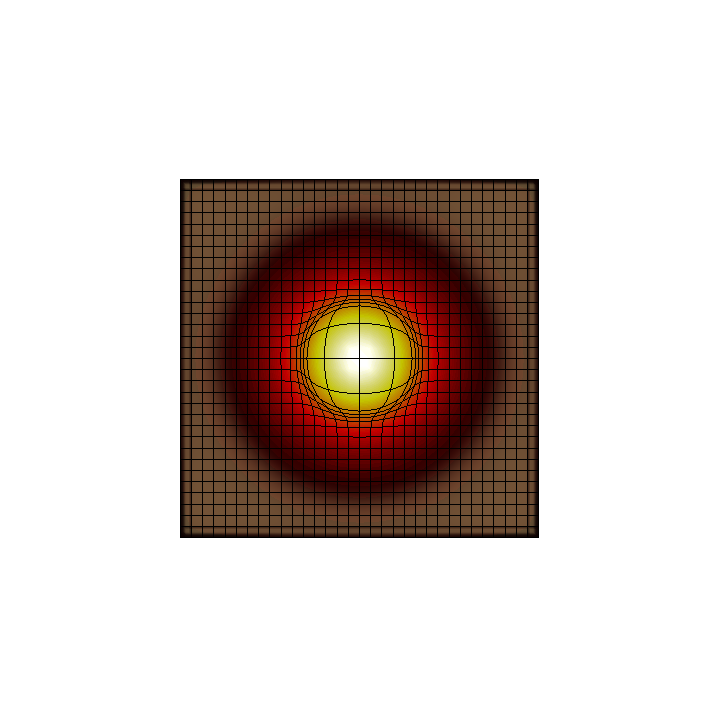
\includegraphics[width=0.3\textwidth]{../figures/ALE_Te_nonlocal32_nopfire.png}
%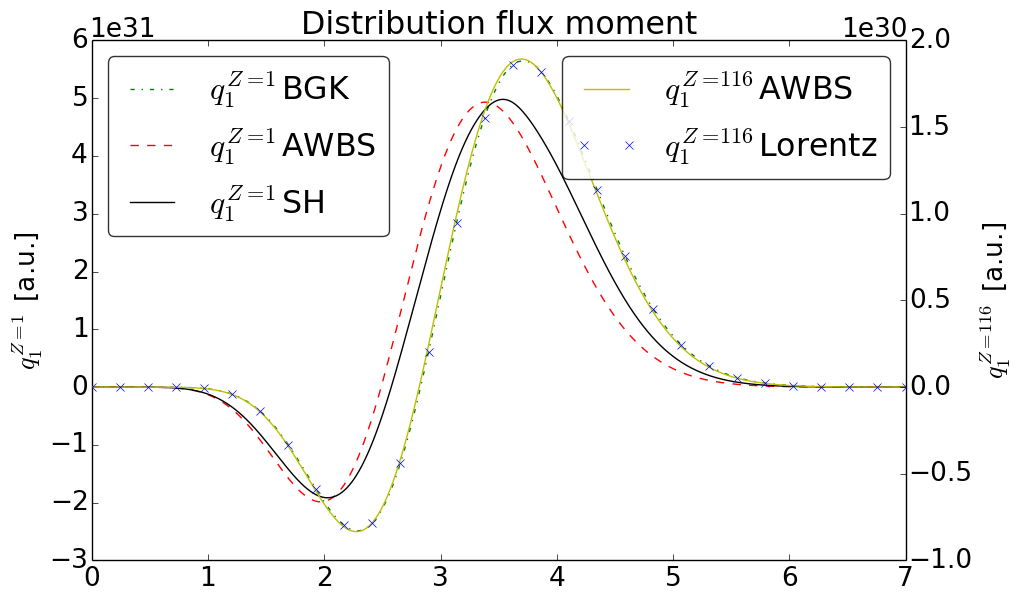
\includegraphics[width=0.3\textwidth]{../figures/q1s.png} &
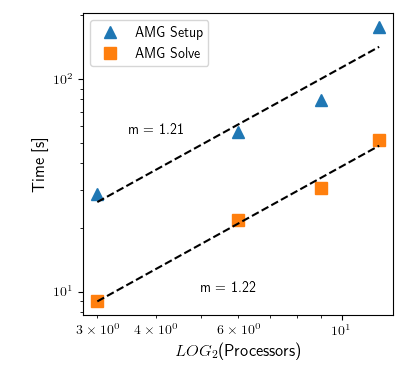
\includegraphics[width=0.3\textwidth]{../figures/pAIR_scaling.png}
\end{tabular}

\end{center}
\end{frame}

\begin{frame}
\begin{center}
{\Huge Nonlocal Ohm's law}

We found that the~quality of the~electric field evaluation is essential for 
a~correct plasma modeling 
\begin{block}{Nonlocal current in plasma}
\begin{equation}
  \vect{j}(f, \vect{E}) = e \int v \fone v^2~\dI v = 
  e \int v \frac{\nuei^2 \vect{E}^* 
  + \omegaB~\omegaB\cdot\vect{E}^* + \nuei~\omegaB \times \vect{E}^*}
  {\nuei (\omegaB^2 + \nuei^2)} v^2~\dI v ,
  \label{eq:NonlocalOhm}
\end{equation}
\end{block}
where $\vect{E}^* = \vmag\frac{\nue}{2}\pdv{\fone}{\vmag} 
- \vmag\nabla\cdot\matr{f}_2 
 - \frac{\qe}{\me}\E\pdv{\fzero}{\vmag}$ 
is an effective electric field in plasma. 
A~comparison to the \textit{Generalized Ohm's law} shows a~correct local 
behavior of \eqref{eq:NonlocalOhm}, especially that 
$\nabla\times \nabla\cdot\matr{f}_2 
\sim \nabla\times \frac{\nabla p_e}{\ed} \sim \nabla n_e \times \nabla T_e$

\begin{block}{Generalized Ohm's law vs. nonlocal Ohm's law}
\begin{eqnarray} 
  \vect{E} &=&  
  \left(\vect{R}_T -\nabla p_e\right)\quad + ~~~~~\quad\qquad 
  \frac{\vect{j}}{\sigma}\qquad\quad ~~~~+
  \qquad \vect{j}\times\vect{B} ,
  \nonumber \\
  \vect{E} \vmag \frac{\qe}{\me}\pdv{\fzero}{\vmag} 
  &=& 
  ~~~~\vmag^2 \nabla\cdot\matr{f}_2 ~~~~~~ 
  +~~~  \vmag^2 \frac{\nue}{2}\pdv{\fone}{\vmag} - \vmag \nuei\fone 
  ~~~+~~~ v \fone\times\frac{\qe}{\me c}\vect{B}.
  %\vect{E} \int v \pdv{\fzero}{v} v^2\, \dI v 
  %&=& 
  %\int v^2 \nabla \fzero v^2\, \dI v~~~ +~~  \int v \nuei\fone v^2\, \dI v 
  %~~~+~~ \int v \fone\times\vect{B} v^2\, \dI v .
  \nonumber
\end{eqnarray}
\end{block}

\end{center}
\end{frame}

\begin{comment} % NonlocalRadHydro
\begin{frame}
\begin{center}
{\large Thermal Radiative Transfer}
\begin{block}{Radiation transport equation}
The~radiation intensity $I_\nu(\vect{x}, \vect{n})$ representing photons of frequency $\nu$ obeys the~equation
\begin{equation}
  \vect{n}\cdot\nabla I_\nu = \eta_\nu - \chi_\nu I_\nu , 
  \nonumber \label{eq:RT}
\end{equation}
where \textit{emmisivity} $\eta_\nu(\rho, T)$ and absorptivity 
$\chi_\nu(\rho, T)$ are considered to be isotropic.
\end{block}
\begin{eqnarray}
  \nabla \cdot \vect{q}_\nu &=& 4\pi\eta_\nu - \chi_\nu E_\nu  \nonumber \\
  \nabla \cdot \matr{P}_\nu &=& -\frac{\chi_\nu}{c}\vect{q}_\nu \nonumber
\end{eqnarray}
\begin{block}{Radiation diffusion}
In the~case of low anisotropy pressure tensor can be approximated as
$\matr{P}_\nu = \matr{I} f_\nu E_\nu$ and the~radiation field can be modeled by
\begin{equation}
  \nabla \cdot \left( \frac{c}{\chi_\nu} \nabla ( f_\nu E_\nu) \right) = 
  \chi_\nu E_\nu - 4\pi\eta_\nu , 
  \nonumber
\end{equation}
where the~lowest anisotropy approximation 
$\tilde{I}_\nu(\vect{x}, \vect{n}) = I^0_\nu(\vect{x}) 
+ \vect{n}\cdot\vect{I}^1_\nu(\vect{x})$ 
corresponds to the~\textit{variable Eddington factor} 
$f_\nu = \frac{1}{3}$.
\end{block}
\end{center}
\let\thefootnote\relax\footnote{D. Mihalas and B. Mihalas, Foundations of Radiation Hydrodynamics 
(Oxford University Press, New York, 1985).}
\end{frame}

\subsection{Nonlocal Magneto-Hydrodynamic model}
\begin{frame}
\begin{center}
{\large Nonlocal Magneto-Hydrodynamic model}
%\myheading{Radiative Fluid Model of Laser Plasma}
%Conservation of mass $\rho$, momentum $\rho \vect{u}$, 
%and energy $\varepsilon_e+\varepsilon_i+\epsilon_R$ of radiation field 
%and plasma fluid, 
%where the inverse-bremsstrahlung deposition of laser electric
%field $\vect{E}_L$ heats the target, read 
\begin{eqnarray}
 \frac{\dI \rho}{\dI t} &=& - \rho\nabla\cdot\vect{u}\, , 
 \nonumber\\ 
 \rho\, \frac{\dI \vect{u}}{\dI t} &=& - \nabla (p_i + p_e + p_{\vect{B}}) \, , 
 \nonumber\\   
 \rho \left(\frac{\partial \varepsilon_i}{\partial T_i}\frac{\dI T_i}{\dI t} 
 +\frac{\partial \varepsilon_i}{\partial \rho}\frac{\dI \rho}{\dI t}\right)
 &=& 
 - p_i\nabla\cdot\vect{u} - G(T_i - T_e)\, , 
 \nonumber\\
 \rho \left(\frac{\partial \varepsilon_e}{\partial T_e}\frac{\dI T_e}{\dI t}
 +\frac{\partial \varepsilon_e}{\partial \rho}\frac{\dI \rho}{\dI t}\right)
  %+ \frac{\dI \epsilon_R}{\dI t} 
  &=& 
 - p_e \nabla\cdot\vect{u} - \nabla\cdot\left(\vect{q}_e+\vect{q}_R \right) + 
 G(T_i - T_e) + Q_{\text{IB}}(\vect{E}_L)\, , 
 \nonumber
\end{eqnarray}
the quantities $\frac{\partial \varepsilon}{\partial \rho} =
\frac{\partial f}{\partial \rho}
- T \frac{\partial^2 f}{\partial \rho \partial T}$, 
$\frac{\partial \varepsilon}{\partial T} = 
-T \frac{\partial^2 f}{\partial T^2}$, 
$p = \rho^2 \frac{\partial f}{\partial \rho}$, 
$G = \rho\frac{\partial \varepsilon_e}{\partial T_e} \nu_{ei}$ 
provides our HerEOS equation of state.
\footnote{M. Zeman, M. Holec, P. Vachal, "HerEOS: a Framework for Consistent Treatment of the Equation of State in ALE Hydrodynamics",\\ 
\textit{Comp. Math. Appl.}, submitted (2017).}
%and depend on ion and electron free energies $f_i(\rho, T_i)$, 
%$f_e(\rho, T_e)$ locally. 

\begin{tabular}{c|c}
\hline \\

\begin{pcolumn}{0.42}
Nonlocal transport of photon intensity 
$I^p=\int_\nu f^p\, \frac{h^4\nu^3}{c^2}\, \dI\nu$
\begin{equation}
  %\frac{1}{c}\frac{\partial I^p}{\partial t} + 
  \vect{n}\cdot\nabla I^p = 
  \frac{a T_e^4 - I^{\, p}}{\lambda^p}\,  \label{photon_transport_equation} 
  \nonumber
\end{equation}
%Photon transport equation using Bhatnagar-Gross-Krook collision operator and related closure via radiation energy density
%and radiation energy density flux for hydro
Radiation closure relations
\begin{equation}
  %\epsilon_R &=& \frac{1}{c}\int_{4\pi} I^{\, p}\, \dI\vect{n}\, \nonumber \\ 
  \vect{q}_R = \int_{4\pi}\vect{n}\, I^{\, p}\, \dI\vect{n}
  \xrightarrow{diffusive} \nabla\cdot\vect{q}_R  = 
  - \nabla\cdot\left( \frac{c}{3 \chi_R}\, \nabla E\right) 
  \,  \nonumber\label{rad_momentum} 
  %\matr{P} &=& \frac{1}{c}\int_{\nu}\int_{4\pi}\vect{n}\vect{n}\, \cInun\, \dI\vect{n}\, \dI\nu\, , \label{rad_stress} 
\end{equation}
\end{pcolumn}
&
\begin{pcolumn}{0.5}
Nonlocal transport of electrons
\begin{equation}
  %\frac{1}{|\vect{v}|}\frac{\partial f}{\partial t} + 
  \vect{v}\cdot\nabla_{\vect{x}} f +
  \left( \vect{E} + \vect{v}\times\vect{B}\right)\cdot\nabla_{\vect{v}} f
  = 
  v \frac{\nu_e}{2} \frac{\partial }{\partial v}\left(f - f_{MB}(T_e)\right)
  + \left(\nu_{ei} + \frac{\nu_e}{2}\right) \left(f_0 - f\right)
  \nonumber
\end{equation}
%Photon transport equation using Bhatnagar-Gross-Krook collision operator and related closure via radiation energy density
%and radiation energy density flux for hydro
Electron closure relations
\begin{eqnarray}
  %\varepsilon^e &=& \frac{1}{\bar{|\vect{v}|}}\int_{4\pi} I^e\, \dI\vect{n}\, 
  %\nonumber \\ 
  \vect{q}_e &=& \int\int_{4\pi}\vect{n}\, f^e\, \dI\vect{n}v^5\, \dI v\, 
  \xrightarrow{diffusive} \nabla\cdot\vect{q}_e = 
  - \nabla\cdot\left(\kappa_{SH}\, T_e^{\frac{5}{2}}\, \nabla T_e\right) 
  \nonumber
  \\
  \vect{j} &=& C(\vect{E}, f)
  \xrightarrow{diffusive} \vect{j} = \sigma_e \vect{E}
  \nonumber
  %\\
  %\vect{Kn}^e &=& \frac{\lambda^e \nabla T_e}{T_e}
  %\nonumber 
  %\\
  %\vect{E} &=& \frac{k_B T_e}{q_e}\frac{5}{2}\frac{\nabla T_e}{T_e}
  %\nonumber
  %\matr{P} &=& \frac{1}{c}\int_{\nu}\int_{4\pi}\vect{n}\vect{n}\, \cInun\, \dI\vect{n}\, \dI\nu\, , \label{rad_stress} 
\end{eqnarray}
\end{pcolumn}
\\ \\\hline
\end{tabular} 
\begin{equation}
  \nabla\times\vect{E} = -\frac{1}{c}\frac{\partial \vect{B}}{\partial t},
  \quad
  \nabla\times\vect{B} = \frac{4\pi}{c} \vect{j}
  \nonumber
\end{equation}
\end{center}
\end{frame}
\end{comment} % NonlocalRadHydro

\begin{comment} % CurvelinearHydro
%\section{Nonlocal-MHD code PETE}
\subsection{Hydrodynamics on curvilinear meshes}
%\begin{comment} % RT pics
\newcommand{\RThscale}{0.9}
\begin{frame}
\begin{center}
%{\large Lagrangian High-Order Curvilinear Framework}

 %New generation high-order curvilinear hydrodynamic code
\begin{tabular}{cc}
 \begin{pcolumn}{0.5}
 \begin{varblock}[0.85\textwidth]{Lagrangian High-Order Curvilinear Framework}
 %High-order finite element discretization introduced by 
 %Dobrev, Kolev, and Rieben 
 %
 %Semidiscrete formulation of Euler's equations in Lagrangian frame, 
 %i.e. momentum, energy, and mass conservation, respectively.
 \begin{eqnarray}
   \matr{M}_{\vect{v}}\cdot\frac{\dI \vect{v}}{\dI t} &=& 
     - \matr{F}\cdot\matr{I} \nonumber \\
   \matr{M}_{e}\cdot\frac{\dI \vect{e}}{\dI t} &=& \matr{F}^T\cdot\vect{v} 
     \nonumber \\
   \frac{\dI \vect{x}}{\dI t} &=& \vect{v} \nonumber \\
   \nonumber 
 \end{eqnarray} 
 \let\thefootnote\relax\footnote{Dobrev, Kolev, Rieben, SIAM JSC 34, B606 (2012).}
 \end{varblock}
 \begin{eqnarray}
   \nonumber  
   \\\nonumber\\\nonumber\\\nonumber\\\nonumber\\\nonumber\\\nonumber
   \\\nonumber\\\nonumber\\\nonumber\\\nonumber\\\nonumber\\\nonumber
   \\\nonumber\\\nonumber\\\nonumber\\\nonumber\\\nonumber\\\nonumber
   %\\\nonumber\\\nonumber\\\nonumber\\\nonumber\\\nonumber\\\nonumber
 \end{eqnarray} 
 \end{pcolumn} &
 \includegraphics<1>[height=\RThscale\textheight]{../../figs_NTH/RT_figs/merged_GLVis_s01.png}
 \includegraphics<2>[height=\RThscale\textheight]{../../figs_NTH/RT_figs/merged_GLVis_s20.png}
 \includegraphics<3>[height=\RThscale\textheight]{../../figs_NTH/RT_figs/merged_GLVis_s40.png}
 \includegraphics<4>[height=\RThscale\textheight]{../../figs_NTH/RT_figs/merged_GLVis_s59.png}
\end{tabular}
\end{center}
\end{frame}
\end{comment} % CurvelinearHydro

\begin{comment} % Ali
\begin{frame}
\begin{center}
{\Huge \textit{Nonlocal-MHD} $\iff$ aiming HIGH}

\begin{tabular}{c}
\includegraphics<1>[width=0.4\textwidth]{../figures/Ali_aiming_high.png}
\includegraphics<2>[width=0.7\textwidth]{../figures/getting_high.png}
\includegraphics<3>[width=0.4\textwidth]{../figures/being_high.png}
\end{tabular}

Height 250 m, overhang 40 m, Visera, Riglos, Spain.

\end{center}
\end{frame}
\end{comment} % Ali

\end{document}
